\chapter{Implementation einer AR Anwendung für Android}
Im Rahmen des Praxisteils dieser Arbeit ist eine Applikation für Android basierte Smartphones erstellt worden. In diesem Praxisteil werden die verwendeten Tools und Frameworks, um die Augmented Reality Anwendung zu erstellen, beschrieben. Das im folgenden vorgestellte Framework ARCore, implementiert den Simultaneous Location and Mapping Ansatz und ist als einzige AR-Programmierschnittstelle Open Source (Siehe Tabelle S.29).



\section{ARCore}
ARCore, das von Google entwickelt wird und das seit März 2018 verfügbar ist, ist der Nachfolger des ebenfalls von Google ins Leben gerufene Projekt Tango, welches jedoch spezielle \glqq Time-of-flight\grqq{} (TOF) Kameras benötigt, um Distanzen im Raum mithilfe des Lichtlaufzeitverfahrens zu messen. Dieser Ansatz hat sich wegen der fehlenden technischen Voraussetzungen der meisten Android Geräte nicht durchgesetzt. Da Google mit dem von Apple veröffentlichen Framework ARKit gleichziehen wollte, wurde Projekt Tango beendet und durch ARCore ersetzt. ARCore verwendet drei Schlüsselfunktionen um virtuelle Objekte in die reale Welt zu integrieren (vgl. \cite{arcore}):

\begin{itemize}
\item \textbf{Motion Tracking} ermöglicht es dem Smartphone seine Position relativ zur Umgebung zu verfolgen und zu verstehen.

\item \textbf{Environmental understanding} ermöglicht es dem Smartphone die Größe und Lage aller Arten von Oberflächen  zu erfassen, dazu zählen horizontale, vertikale oder schräge Oberflächen.

\item \textbf{Light estimation} ermöglicht die Abschätzung der aktuellen Lichtverhältnisse in der Umgebung, zur korrekten Beleuchtung und zur Erstellung von Schatten.
\end{itemize}

\subsection{Unterstütze Geräte}
Um eine gute und flüssige Erfahrung für den Endnutzer zu gewährleisten, müssen unterstützte Smartphones bestimmte Kriterien erfüllen. Dazu zählen die Qualität der verbauten Kamera, der Bewegungssensoren und der Designarchitektur. Weiterhin muss das Gerät über eine leistungsstarke CPU verfügen, die sich in das Hardware-Design integriert, um gute Leistung und effektive Echtzeitberechnung zu gewährleisten. Die Voraussetzungen um ARCore zu verwenden, werden wie folgt definiert:

\begin{itemize}
\item \textbf{Android 7.0} oder höher (Einige Modelle benötigen neuere Versionen).
\item Ein Gerät, das ursprünglich mit dem \textbf{Google Play Store} ausgeliefert wurde.
\item \textbf{Internetzugang}, um Google Play Services für AR zu installieren oder zu aktualisieren.
\end{itemize}

Aktuell werden 144 Android Smartphones, die mit dem Google Play Store ausgeliefert werden unterstützt. Weiterhin werden 29 chinesische Modelle unterstützt, bei welchen die Google Play Services manuell über die App Stores der Hersteller installiert werden müssen. Auch 20 iOS Smartphone Modelle werden unterstützt, dabei benötigt ARCore jedoch ARKit kompatible Geräte mit iOS 11.0 oder höher (Stand 22.08.2019, vgl. \cite{arcore_devices}).

\subsection{Grundlegende Konzepte}

In diesem Abschnitt werden grundlegende Funktionen, die ARCore bietet, erläutert.

\textbf{Motion Tracking} wird in ARCore mit einem Prozess namens \glqq Concurrent Odometry and Mapping\grqq{} (COM) ermöglicht. Dabei werden Features im Kamerabild erkannt und zur Bestimmung der Änderung der Position des Smartphones verwendet. Diese visuellen Informationen werden mit Trägheitsmessungen der internen Messeinheiten (IMU) des Smartphones kombiniert, um die Position und Ausrichtung der Kamera relativ zur Umwelt zu bestimmen.

Google hat sich das System und die Methodik hinter \glqq Concurrent Odometry and Mapping\grqq{} patentieren lassen. Die Beschreibung des Patents und des Systems hinter COM zeigt viele Zusammenhänge des implementierten Systems in ARCore mit SLAM und photogrammetrischen Verfahren (vgl. \cite{patent}): 

\glqq \textit{An electronic device tracks its motion in an environment while building a three-dimensional visual representation of the environment that is used to correct drift in the tracked motion. A motion tracking module estimates poses of the electronic device based on feature descriptors corresponding to the visual appearance of spatial features of objects in the environment. A mapping module builds a three-dimensional visual representation of the environment based on a stored plurality of maps, and feature descriptors and estimated device poses received from the motion tracking module. The mapping module provides the three-dimensional visual representation of the environment to a localization module, which identifies correspondences between stored and observed feature descriptors. The localization module performs a loop closure by minimizing the discrepancies between matching feature descriptors to compute a localized pose. The localized pose corrects drift in the estimated pose generated by the motion tracking module.}\grqq{}

Auch die Abbildungen über die Pipeline von COM zeigen eine hohe Übereinstimmung mit der photogrammetrischen Pipeline, sowie gegenüber SLAM, siehe Abb. 6.1.

\begin{figure}[H]
	\centering
	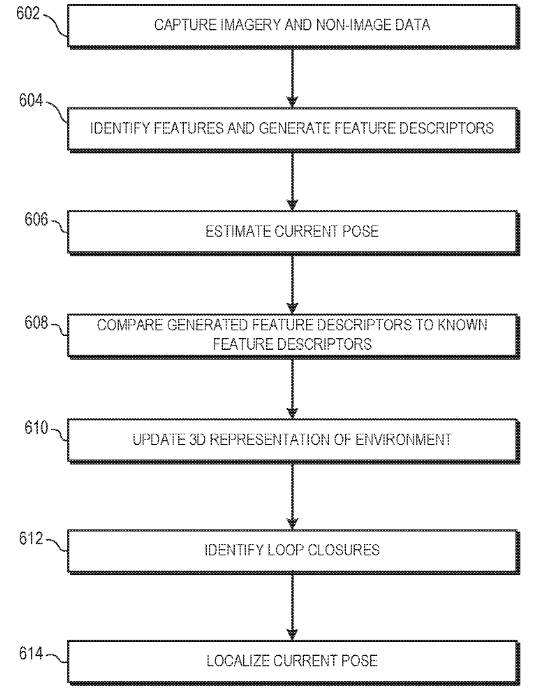
\includegraphics[scale=0.75]{com.png}
	\caption{Pipeline von COM. Bildquelle \cite{patent}}
\end{figure} 


\textbf{Environmental Understanding} wird in ARCore durch die Erkennung von Clustern von Feature Punkten auf üblichen horizontalen oder vertikalen Flächen ermöglicht. Weiterhin können die Grenzen dieser Ebenen bestimmt werden. Da ARCore zur Erkennung der Ebenen Features verwendet, werden flache oder texturlose Oberflächen, wie beispielsweise eine weiße Wand möglicherweise nicht richtig erkannt. 

\textbf{Light Estimation} wird in ARCore verwendet, um Informationen über die Beleuchtung der Umgebung zu erhalten. Dazu werden Daten wie durchschnittliche Intensität der Helligkeit oder Farbtemperatur erfasst. Anhand dieser Informationen kann mit einer Helligkeitsanpassung oder Farbkorrektur das Gefühl von Realismus in der Szene verstärkt werden, indem virtuelle Objekte unter den gleichen Bedingungen wie die echte Welt beleuchtet werden.

\textbf{User Interaction} wird in ARCore mit Hilfe von \glqq Hit-testing\grqq{} ermöglicht. Eine $(x,y)$ Koordinate auf dem Bildschirm des Smartphones wird mithilfe eines Strahls (Ray) in das Kamerabild projiziert. Alle Schnittpunkte mit Ebenen oder Merkmalspunkten des Strahls werden zusammen mit der Pose dieses Schnittpunktes zurückgegeben. Dadurch können Nutzer mit virtuellen Objekten interagieren.

\textbf{Anchors und Trackables} (Anker und trackbare Objekte) werden verwendet, da sich die Positionen von Flächen verändern kann, wenn ARCore im Lokalisierungsprozess das Verständnis für die eigene Position und das Umfeld verbessert. Um ein virtuelles Objekt zu platzieren, muss ein Anker erstellt werden, um sicherzustellen, dass ARCore die Position dieses Objekts über die Zeit verfolgt. Ebenen und Punkte sind hier eine spezielle Art von Objekt, das als \glqq Trackable\grqq{} bezeichnet wird. Virtuelle Ojekte können an bestimmten Trackables verankert werden, um sicherzustellen, dass die Beziehung zwischen virtuellen Objekt und dem zu verfolgenden Punkt oder Ebene stabil bleibt, auch wenn sich das Gerät bewegt. Das heißt, dass virtuelle Objekte, die beispielsweise auf einem gewissen Punkt am Boden platziert werden, immer noch auf exakt der gleichen Position bleiben, auch wenn die Ebene, die den Boden repräsentiert, durch ARCore angepasst und verschoben wird.

\textbf{Augmented Images} ist eine Funktion, mit der Augmented Reality Anwendungen erstellt werden können, die auf bestimmte 2D-Bilder, wie beispielsweise Produktverpackungen oder Filmposter reagieren können.

\begin{figure}[H]
	\centering
	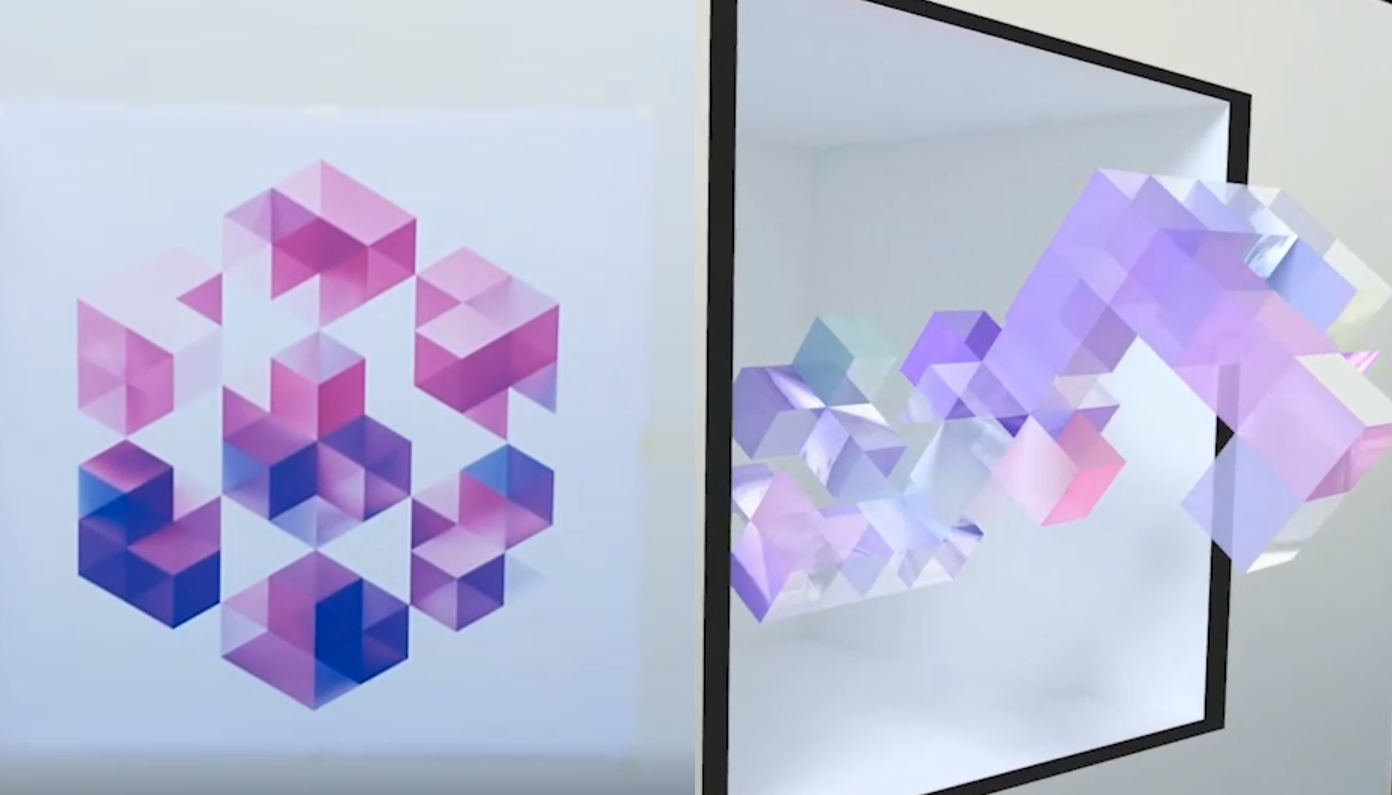
\includegraphics[scale=0.4]{augmented.png}
	\caption{Augmented Image mit ARCore, Bildquelle \cite{augmented_images}}
\end{figure} 

ARCore bietet auch eine Funktion um bewegende Bilder zu verfolgen, wie beispielsweise eine Plakatwand, auf der Seite eines fahrenden Busses. Die Bilder können offline zusammengestellt werden, um eine Bilddatenbank zu erstellen, es ist jedoch auch möglich einzelne Bilder in Echtzeit vom Gerät hinzuzufügen. Nach der Registrierung erkannt ARCore diese Bilder, sowie die Grenzen dieser und gibt eine entsprechende Pose eines virtuellen Objekts zurück.

Mithilfe der \textbf{ARCore Cloud Anchor API} können kollaborative AR Multiplayer Anwendungen erstellt werden. Dazu wird von einem Gerät der Anker und die Features der näheren Umgebung in der Cloud gespeichert. Diese Anker können dann mit anderen Benutzern auf Android- oder iOS-Geräten in der selben Umgebung geteilt werden. Mit dieser Methode können zwei Endgeräte die gleiche virtuellen 3D Objekte an exakt der gleichen Stelle im Raum rendern, so dass beide Benutzer das gleiche Erlebnis teilen (vgl. \cite{fundamental_concepts}).

\subsection{Entwicklungsumgebungen}

ARCore kann mit vielen gängigen Entwicklungsumgebungen verwendet werden. Dazu zählen Android Studio, Android Native Development Kit, Unity für Android, Unity für iOS, Unreal Engine und iOS (vgl. \cite{develop}). Im Rahmen dieser Arbeit wurde Android Studio in der Version 3.4.1, sowie ARCore in der Version 1.11.0 verwendet.

\section{Sceneform}
Sceneform ist eine Framework, das von Google entwickelt wurde und welches nahtlos in ARCore integriert werden kann. Es ermöglicht das einfache Rendern von realistischen 3D-Szenen in AR- und Nicht-AR-Anwendungen, ohne auf OpenGL zurückgreifen zu müssen. Sceneform bietet folgende Features (vgl. \cite{sceneform}):

\begin{itemize}
\item Einen high-level \textbf{Szenengraph API}.
\item Einen realistischen \textbf{physikalischen Renderer} namens \textbf{Filament}.
\item Ein \textbf{Android Studio-Plugin} zum Importieren, Anzeigen und Erstellen von \textbf{3D-Assets}.
\end{itemize}

Sceneform benötigt Android Studio Version 3.1 oder höher und wird als Plugin installiert. Es liefert ein sogenanntes \glqq ArFragment\grqq{} welches automatisch das ARCore Session Management übernimmt, sowie die notwendigen ARCore Laufzeitprüfungen durchführt. Dazu gehört die automatische Überprüfung von kompatiblen Versionen der Google Play Services für Augmented Reality und die Überprüfung der Berechtigung für Kamera und anderer Sensoren. Sind alle Überprüfungen erfolgreich, erstellt das ArFragment eine \glqq ArSceneView\grqq{} und eine ARCore Session. Mithilfe der ArSceneView kann nun das Kamerabild gerendert werden, sowie mithilfe eines \glqq PlaneRenderers\grqq{} die erkannten Ebenen zur Platzierung von virtuellen Objekten visualisert werden.

Der ArSceneView ist eine Szene zugeordnet, welche eine baumartige Datenstruktur beinhaltet. Die Nodes dieser Datenstruktur sind die zu rendernden virtuellen Objekte. Jedes Node enthält alle Informationen, um es zu rendern und damit zu interagieren. Dazu gehören Position, Ausrichtung, Modell, Kollisionsform und Event Listener. Nodes können mit anderen Nodes Eltern-Kind-Beziehungen formen, welche sich in einer baumartigen Struktur kristallisieren. Diese Struktur wird dann als Szenengraph bezeichnet. Bei jedem Einzelbild rendert Sceneform den Szenengraph aus Sicht der Kamera, welche durch das ARCore Tracking geführt wird (vgl. \cite{sceneform_google}). 

Filament ist eine physikalisch basierte Rendering (PBR) Engine für Android, die ihren Fokus auf Echtzeit Performance bei mobilen Geräten legt. Das Hauptziel von Filament sind GPUs der Klasse OpelGL ES 3.x. Die Hauptgesichtspunkte der Engine liegen in den Bereichen Qualität, Benutzerfreundlichkeit, Vertrautheit, Flexibilität und in der Größe der bereitgestellten Renderbibliothek. Physikalisch basiertes Rendering ist ein Verfahren, das eine genauere Darstellung von Materialien und deren Wechselwirkungen mit Licht im Vergleich zu herkömmlichen Echtzeitmodellen ermöglicht. Die Trennung von Materialien und Beleuchtung im Kern der PBR Methode macht es einfacher, realistische Objekte zu erstellen, die unter allen Lichtverhältnissen präsize aussehen (vgl \cite{filament}).


\section{Google Places API}

Im Rahmen dieser Arbeit wird die Google Places API, zur Abfrage von Informationen mithilfe des aktuellen Standort des Smartphones, verwendet. Die Places-API ist ein Dienst, der Informationen über bestimmte Orte mit HTTP-Anfragen zurückgibt. Places sind innerhalb der API definiert als Einrichtungen, geografische Standorte oder berühmte Points of Interest. Die Informationen die mit der API abgefragt werden können, sind etwa einfache Listen der näheren Orte, Details über die Orte in der Nähe oder Fotos der näheren Orte, aus der Google Datenbank. Die API ermöglicht auch die  Autovervöllständigung von Suchanfragen bestimmter Orte oder Querys. Jeder dieser Dienste wird als HTTP-Request aufgerufen und gibt entweder XML- oder JSON-Dateien als Antwort zurück. Alle Anfragen müssen das HTTPS Protkoll verwenden und benötigen einen eigenen API Schlüssel (vgl. \cite{places_api}).

Bei der Implementation der App wurde die \glqq Place Search\grqq{} Funktion der API verwendet. Ein Call schaut wie folgt aus:

\begin{lstlisting}[basicstyle=\small]
https://maps.googleapis.com/maps/api/place/nearbysearch/json?location=
 + LAT_LNG + &rankby=distance&keyword= + KEY_WORD + &key= + API_KEY;
\end{lstlisting}

Das Ergebnis dieses Anfrage Querys erhält eine Vielzahl an Informationen, die anschließend weiter verarbeitet werden können.





\section{Dexter}

\section{Volley}

\section{Implementierung}



